
\msection{\Wasm}

The Web Consortium (W3C) standardized in 2017 a bytecode for the web environment, the \Wasm language. 
% Describe WebAssembly
Wasm is designed to be fast, portable, self-contained, and secure \cite{Haas_2017}.
All Wasm programs are compiled ahead-of-time from source languages such as C/C++ and Rust.
All major browser vendors have adopted \Wasm as a standard for web applications.
Moreover, WebAssembly has been evolving outside web browsers since its first announcement.


Some works demonstrated that using WebAssembly as an intermediate layer is better in terms of startup and memory usage than containerization and virtualization \cite{pMendkiServerless, 1244493Jacobsson}. 
Consequently, in 2019, the Bytecode Alliance \cite{bytecodealliance} proposed WebAssembly System Interface (WASI) \cite{WASI}. 
WASI pionered the execution of \wasm\ with a POSIX system interface protocol, making possible to execute Wasm directly in the operating system. 
Therefore, it standardizes the adoption of \wasm\ in heterogeneous platforms \cite{bryant2020webassembly}, making it suitable for edge-cloud computing platforms \cite{9640153, wen2020wasmachine}
In the subsequent sections we describe the \wasm\ language, its execution model, and its ecosystem.

\msubsection{Binary format}
\label{background:wasm:binary}

\begin{table}
    \centering
    \begin{tabular}{r l | p{8cm}}
        ID & Section Name & Description \\
        \midrule
        0 & Custom & It is a compound of two parts, the name of the section followed by arbitrary content. It is mostly used to store metadata of the \wasm program such as the compiler that generates the binary. \\
        \hline
        1 & Type & Function signatures of the functions declared or defined inside the binary. \\
        \hline
        2 & Import & Imported elements from the host such as: functions, memories, globals and tables. \\
        \hline
        3 & Function & Functions defined inside the binary. It is basically a map between the Type section entries and the code entries defined in the Code section.  \\
        \hline
        4 & Table & Contains groups of functions that follow the same signature. It is used to control indirect calls. \\
        \hline
        5 & Memory & Defines the number of unmanaged linear memories along with its initial size.\\
        \hline
        6 & Global & Defines global variables are managed memory to be used and shared between functions in the \wasm binary. \\
        \hline
        7 & Export & Declares functions, globals, memories and tables to be accessed by the host engine. For example, the entry point of the \wasm binary is declared as an exported function. \\
        \hline
        8 & Start & \Wasm can declare a function to be called as soon as the binary is ready for execution. It serves to initialize the state of the \wasm program previous to the execution of any of its exported functions. \\
        \hline
        9 & Element & List of elements to initialize the binary tables \todo{Check this} \\
        \hline
        10 & Code & Body of defined functions in the Function section. Each entry is a compound of the used local variables and the function body. The latter one is a list of instructions. \\
        \hline
        11 & Data & Data used to initialize the unmanaged linear memory. Each entry contains the offset and the data that should be placed in the linear memory. \\
        \hline
        12 & Data Count & It is mostly used to validate the Data Section of the binary. If the number of segments declared in the Data Section does not match with the Data Count section, the binary is malformed.\\
    \end{tabular}
    \caption{Binary section of \Wasm binaries following \wasm 1.0 specification.}
    \label{background:wasm:sections}
\end{table}


A Wasm binary has a unique module as its main component, serving as the fundamental unit of deployment, loading and compilation of a \Wasm program.
A module is composed of sections, corresponding to 13 types\footnote{\url{https://webassembly.github.io/spec/core/binary/modules.html\#sections}}, each of them with an explicit semantic and a specific order inside the module. 
This makes the compilation to machine code faster. 
In \autoref{background:wasm:sections} we summarize the sections of a Wasm  binary.
Each table entry contains: the section ID, the name of the section, and a brief description of its purpose. 

\begin{figure}
    \centering
    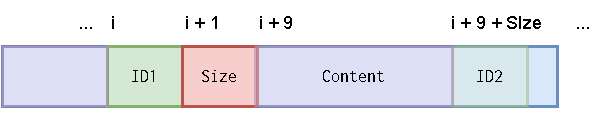
\includegraphics[width=0.5\linewidth]{figures/section.pdf}
    \caption{Wasm binary section. It starts with the section ID followed by the section size and the section content.}
    \label{background:wasm:fig:section}
\end{figure}

\todo{Recheck this}
In \autoref{background:wasm:fig:section} we illustrate the memory bytes representation of a \wasm section.
A \wasm section is a collection of bytes that starts with 1 byte annotating the ID of the section. 
Then 8 bytes follows annotating the size of the section in bytes. 
Finally, the content of the section follows with exactly the size annotated in the previous step.  

% The order of the sections sometimes does not matter, neither their presence
Some sections in the binary are optional, such as the Start section, which is not mandatory to be present in the binary.
The same applies to the Custom sections, which is used to store metadata of the binary, such as the compiler that generates the binary.
Given the previously mentioned section format inside the binary, it is possible to skip sections by just ignoring the bytes that correspond to the section.
This makes the processing of \wasm (for example compiling) faster, as the compiler does not need to parse the whole binary to find the section it is looking for.
On the other hand, the only order constraint is related to a few sections, not all. 
This means that the order of the sections is not important in some specific cases.
Moreover, sections could be repeated in the binary, such as the Data section, which can be repeated as many times as the user wants.

\msubsection{Memory model}
\label{background:wasm:memory}
\todo{Managed and unmanaged}


% Memory, globals and functions
Wasm  manages the memory in a restricted way. A Wasm  module has a linear memory component that is accessed with \texttt{i32} pointers (integer of 32 bits) and should be isolated from the virtual stack. The declaration of the linear data in the memory is showed in \lineref{data}. The memory access is illustrated in \lineref{load}. This memory is usually bound in browser engines to 4Gb of size, and it is only shareable between the process that instantiate the Wasm  binary and the binary itself (explicitly declared in \lineref{mem1} and \lineref{export2}). This ensures the isolation of the execution of Wasm  code. 

Wasm  also provides global variables in their four primitive types. Global variables (\lineref{global1}) are only accessible by their declaration index, and it is not possible to dynamically address them. For functions, Wasm  follows the same mechanism, either the functions are called by their index (\lineref{call}) or using a static table of function declarations. The latter allows modeling dynamic calls of functions (through pointers) from languages such as C/C++, for which the Wasm's compiler is in charge of populating the static table of functions.


\msubsection{Execution model}
\label{background:wasm:execution}
\todo{Stack, frames and blocks}
\todo{First order breaks}

Functions, instructions, and variables are statically typed, meaning their types are deter- 
mined at compile time. There exist only four primitive values types: 32-bit and 64-bit integers 
(i32/i64) and single-precision and double-precision floating-point numbers (f32/f64). Aggregate 
types, such as classes, objects, and arrays, are not natively supported. Instead, during compilation, 
such types are transformed into primitive types and stored in memory.

% Example and intro to the stack
In \autoref{CExample} and \autoref{WASMExample} we illustrate a C program and the Wasm program that results from its compilation. The C function contains: heap allocation, external function declaration and the definition of a function with a loop, conditional branching, function calls and memory accesses. The code in \autoref{WASMExample} shows the textual format for the generated Wasm. The module in this case first defines the signature of the functions (\lineref{tpe1}, \lineref{tpe2}  and  \lineref{tpe3})  that help in the validation of the binary defining its parameter and result types. The information exchange between the host and the Wasm  binary might be in two ways, exporting and importing functions, memory and globals to and from the host engine (\lineref{import1}, \lineref{export1} and \lineref{export2}). The definition of the function (\lineref{func1}) and its body follows the last import declaration at \lineref{import1}. 


The WebAssembly runtime structure is described in the WebAssembly specification and it includes 10 key elements: the Store, Stack, Locals, Module Instances, Function Instances, Table Instances, Memory Instances, Global Instances, Export Instances, and Import Instances. These components interact during the execution of a WebAssembly program, collectively defining the state of a program during its runtime.

Two of these elements, the Stack and Memory instances, are particularly significant in maintaining the state of a WebAssembly program during its execution. The Stack holds both values and control frames, with control frames handling block instructions, loops, and function calls. Meanwhile, Memory Instances represent the linear memory of a WebAssembly program, consisting of a contiguous array of bytes.
In this paper, we highlight the aforementioned two components to define, compare and validate the state of two Wasm programs during their execution. 

% Example
\begin{code}
    \begin{minipage}[t]{0.45\linewidth}
        \lstset{language=C,caption={Example C function.},
        label=CExample,
        breaklines=true, 
        basicstyle=\small\ttfamily,
        postbreak=\mbox{\textcolor{red}{$\hookrightarrow$}\space},
        escapeinside={(*@}{@*)}
        }
%\input{sota/code/code.c}
\end{minipage}\hspace{10mm}
\begin{minipage}[t]{0.46\linewidth}
\lstset{
    language=WAT,
    caption={\wasm\ code  for \autoref{CExample}.},
    style=WATStyle,
    breaklines=true, 
    %stepnumber=0,
    escapeinside={(*@}{@*)},
    numbers=left,
    postbreak=\mbox{\textcolor{red}{$\hookrightarrow$}\space},
    label=WASMExample}
%
%\input{sota/code/code.fix.wat}
%\end{lstlisting}
\end{minipage}


%\begin{tikzpicture}[remember picture,overlay]

%\path (2.west) edge[<-, black] (1.west);
%\path (3.west) edge[<-,  black] (4.west);

%\path (6.east) edge[<-, bend right, black] (3.east);
%\path (9.east) edge[<-, bend right, black] (4.east);
%\path (7.east) edge[<-, bend right, black] (8.east);


%\end{tikzpicture}
\end{code}


% Functions
The function body is composed of local-variable declarations and typed instructions that are evaluated using a virtual stack (Line 7 to Line 32 in \autoref{WASMExample}). Each instruction reads its operands from the stack and pushes back the result. The result of a function call is the top value of the stack at the end of the execution. In the case of \autoref{WASMExample}, the result value of the main function is the calculation of the last instruction, \texttt{i32.add} at \lineref{result}. A valid Wasm  binary should have a valid stack structure that is verified during its translation to machine code. The stack validation is carried out using the static types of Wasm, \texttt{i32} for 32 bits signed integer, \texttt{i64} for 64 bits signed integer, \texttt{f32} for 32 bits float and \texttt{f64} for 64 bits float. As the listing shows, instructions are annotated with a numeric type.

In Wasm, all instructions are grouped into blocks, where the start of a function is the root block. Two consecutive block declarations can be appreciated in \lineref{block1} and \lineref{block2} of \autoref{WASMExample}. Control flow structures jump between block boundaries and not to any position in the code like regular assembly code. A block may specify the state that the stack must have before its execution and the result stack value coming from its instructions. Inside the Wasm  binary the blocks explicitly define where they start and end (\lineref{end1} and \lineref{end2}). By design, each block executes independently and cannot execute or refer to outer block codes. This is guaranteed by explicitly annotating the state of the stack before and after the block. Three instructions handle the navigation between blocks: unconditional break, conditional break (\lineref{break1} and \lineref{break2}) and table break. Each break instruction can only jump to one of its enclosing blocks. For example, in \autoref{WASMExample}, \lineref{break1} forces the execution to jump to the end of the first block that starts at \lineref{block1} if the value at the top of the stack is greater than zero.


\todo{Words on version 1.0 and why our tools  have no issues with it.}



% We do not enumerate the types, lets try to be as much agnostic to the version of Wasm as possible
WebAssembly programs operate on a virtual stack that allows primitive data types.
% These same data types are used to annotate instructions in the WebAssembly code.
Additionally, a WebAssembly program might include several custom sections.
For example, binary producers such as compilers use custom sections to store metadata, such as the name of the compiler that generates the Wasm code.
A WebAssembly program also declares memory sections and globals, which are used to store, manipulate and share data during program execution, e.g. to share data with the host engine of the WebAssembly binary.

WebAssembly is designed with isolation as a primary consideration. For instance, a WebAssembly binary cannot access the memory of other binaries or cannnot interact directly with browser's APIs, such as the DOM or the network. Instead, communication with these features is constrained to functions imported from the host engine, ensuring a secure and safe Wasm environment.
Moreover, control flow in WebAssembly is managed through explicit labels and well-defined blocks, which means that jumps in the program can only occur inside blocks, unlike regular assembly code \cite{10.1145/3062341.3062363}. 
%\todo{Change the example to Rust}
In \autoref{example:cprogram}, we provide an example of a Rust program that contains a function declaration, a loop, a loop conditional, and a memory access. When the Rust code is compiled to WebAssembly, it produces the code shown in \autoref{example:wasmprogram}. The stack operations are folded with parentheses.
The module in the example contains the components described previously.


\msubsection{WebAssembly's Ecosystem}
\label{background:wasm:ecosystems}

\todo{Go deep into the details of the tools that are comoing from parts of the jury}

\Wasm programs are pre-compiled from an array of source languages and are designed for execution in host environments such as web browsers.
Though the execution of a \Wasm program might be considered its final lifecycle stage, the \Wasm ecosystem is far from simplistic.
It comprises multiple stakeholders and a rich array of tools that cater to various needs.
In the subsequent text, we describe the \Wasm ecosystem and explore its key stakeholders.

\wrule{Producers}, such as compilers, transform source code into \Wasm binaries. 
For example, LLVM has offered \Wasm as a backend option since its 7.1.0 release\footnote{\url{https://github.com/llvm/llvm-project/releases/tag/llvmorg-7.1.0}}, supporting a diverse set of frontend languages like C/C++, Rust, Go, and AssemblyScript\footnote{A subset of the TypeScript language}.
In parallel developments, the KMM framework\cite{kmm} has incorporated \Wasm as a compilation target, and the Javy approach\cite{Javy} focuses on encapsulating JavaScript code within isolated \Wasm binaries. 
This is achieved by porting both the engine and the source code into a secure \Wasm environment. 
Blazor also enables the compilation of C# code into \Wasm binaries for browser execution\footnote{\url{https://dotnet.microsoft.com/apps/aspnet/web-apps/blazor}}.
Regardless of the source language or framework, the resulting \Wasm binary functions similar to a traditional shared library, replete with code instructions, symbols, and exported functions.
%From a security standpoint, \Wasm programs are designed without a standard library and are prohibited from direct interactions with the operating system. Instead, the host environment offers a predefined set of functions that can be imported into the \Wasm program. 
%It falls upon the producers to specify which functions from the host environment will be imported by the \Wasm application.

\wrule{Consumers} encompass tools that undertake the tasks of validating, analyzing, transpiling to machine code, and executing \Wasm binaries, e.g. browser clients. 
In the text that follows, we dissect them into specific categories and their respective domains of application.

\todo{Locate WasmA} \cite{WasmA}

\wrule{Static and dynamic analysis, optimization and validation:} The toolkit for analysing \Wasm binaries is rich and varied. 
Tools such as Wassail\cite{wassail}, Wasmati\cite{wasmati}, and Wasp\cite{Wasp} utilize a range of methodologies, including information flow control, code property graphs, and concolic execution, to identify vulnerabilities. 
Dynamic analysis counterparts like TaintAssembly\cite{taintassembly}, Wasabi\cite{wasabi}, and Fuzzm\cite{fuzzm} serve analogous functions.
\todo{Add veriwasm}
\todo{Binanryen}

\wrule{Browsers} Engines like V8\cite{v8}, SpiderMonkey\cite{spidermonkey}, and Chakra\cite{chakra} are at the forefront of executing \Wasm binaries. 
These engines leverage Just-In-Time (JIT) compilers to convert \Wasm into machine code. 
This translation is typically a straightforward one-to-one mapping, given that \Wasm is already an optimized format closely aligned with machine code. 
For example, V8 employs quick, rudimentary optimizations such as constant folding and dead code removal\footnote{This analysis was corroborated through discussions with the V8 development team and through empirical studies in one of our contributions\cite{CROW}}. 

\wrule{Standalone engines} \Wasm's applicability has transcended browser environments, largely due to the WebAssembly System Interface (WASI)\cite{WASI}. 
WASI aims to standardize the interaction between host environments and \Wasm modules, thereby facilitating portability of both bytecode and binaries across diverse platforms. 
It outlines a POSIX-like Application Binary Interface (ABI), which includes functionalities for filesystem access, network sockets, clocks, and random number generation, among others. 
Standalone engines such as WASM3\cite{wasm3}, wasmtime\cite{wasmtime}, WAVM\cite{WAVM} and Sledge \cite{Sledge} have emerged to support \Wasm.
Similarly, Singh and colleagues \cite{WARDuino2019} proposed a virtual machine for Wasm in Arduino based devices.


\todo{Disect them into, JIT compilers and interpreters, ending with SWAM.}
\todo{Add the verifiable standalone engine here}

\wrule{Specialized Malware Detection} In niche areas like cryptomalware detection, tools like MineSweeper\cite{Minesweeper}, MinerRay\cite{MinerRay}, and MINOS\cite{MINOS} utilize static analysis techniques. 
Conversely, dynamic analysis is the forte of tools like SEISMIC\cite{SEISMIC}, RAPID\cite{RAPID}, and OUTGuard\cite{outguard}.

\wrule{Smart Contract Analysis} In the field of smart contracts, static analysis tools like EvalHunter\cite{evalhunter}, WANA\cite{wana}, and EOSAFE\cite{eosafe} are employed to unearth vulnerabilities in \Wasm-based contracts. Dynamic analysis tools in this sphere include EOSFuzzer\cite{eosfuzzer} and wasai\cite{wasai}.


\wrule{Obfuscation, and binary rewriting tools} \todo{WASMixer, Wobfuscator}

While many existing tools purport to offer self-correctness evaluations and exhaustive test suites, the \Wasm ecosystem is still in its early stages. 
To emphasize this, a 2021 study by Hilbig et al.\cite{Hilbig2021AnES} found a mere 8,000 unique \Wasm binaries globally. 
This pales in comparison to mature ecosystems like JavaScript and Python, which offer 1.5 million and 1.7 million packages on npm\footnote{\url{https://www.npmjs.com/}} and PyPI\footnote{\url{https://pypi.org/}}, respectively.
This limited pool of \Wasm binaries presents a unique challenge for machine learning-based analysis tools, which require large datasets for effective training. 
This issue is explicitly addressed in one of the contributions of this dissertation\cite{EVASION}.
Additionally, the scarcity of \Wasm programs exacerbates the problem of software monoculture, increasing the likelihood of consuming a compromised \Wasm program\cite{YourCitationHere}.
Besides, the current size of the \Wasm ecosystem offers a small testing environment for evaluating the capabilities of consumer tools.
This dissertation aims to address these issues by introducing a comprehensive suite of tools. 
These tools are crafted to not only bolster the security of \Wasm programs through Software Diversification but also to intensify the testing rigor for both producers and consumers in the ecosystem.


To the best of our knowledge, the most complete survey about Wasm  tooling is presented in the Awesome Wasm  (\url{https://github.com/mbasso/awesome-wasm}) repo. It is a cumulative GitHub repo which includes references to articles, papers, books, demos, compilers and engines related to \wasm. 
